\section{Experiments}
In this section we first introduce the popular ATIS dataset,
and describe how we collect our E-commerce Shopping Guide Assistant (ECSGA) dataset.
Then we show the implementation details for our model.
Finally we demonstrate the evaluation results on both ATIS and ECSGA dataset and give some discussions.
In the following experiments, we call our proposed Deep Cascade Multi-task Learning method as DCMTL for short.

\subsection{Dataset}
\label{sec:data}
\noindent
\textbf{ATIS Dataset:}
The ATIS\footnote{The data can be found at \url{https://github.com/yvchen/JointSLU/tree/master/data}.} corpus is the most commonly used dataset for slot filling research,
which consists of reservation requests from the air travel domain.
%It contains 4,978 training and 893 testing sentences in total, with a vocabulary size of 572.
There are 84 different slot labels (127 with IOB prefix). 
We randomly selected 80\% of the training data for model training and the 
remaining 20\% as the validation set \cite{mesnil2015using}.
Apart from the ground-truth slot labels, we also generate its 
corresponding segment labels for our multi-task model setting.

\noindent
\textbf{ECSGA Dataset:}
To create large amounts of gold standard data 
for the training of our model,
we adopt an unsupervised method to 
automatically tag the input utterances.
All the utterances are extracted from the user input logs 
(either from text or voice) on an online shopping guide 
assistant system.  Our E-commerce knowledge base
is a dictionary consisting of pairs of
word terms and their ground-truth slot labels 
such as ``红色-颜色''\emph{(red-color)}.
%This is a standard resource constructed by human beings,
%so we can use it to create gold standard.
We use a dynamic programming algorithm to 
match terms in the utterances and then assign each word with 
its slot label in IOB scheme.
We filter utterances whose matching result is
ambiguous and only reserve those that can be 
perfectly matched
(all words can be tagged by only one unique label) 
as our training and testing data.
With the slot labels of each word, we can induce the 
named entity labels and segment labels straightforwardly.
%For we only extract the perfectly matched sentences,
%the quality of our ECSGA dataset can be absolutely guaranteed.
Our goal is to develop 
%One may wonder why we can't just use the max-matching algorithm and 
%a good dictionary to do the slot filling itself.
%However the dictionary can only cover or recognize limited sentences.
a sequence labeling algorithm with the ability to generalize to vocabulary
outside of the dictionary.
%In fact, for our online usage we first use a dictionary to apply max-matching algorithm to do tagging,
%and if we cannot tag the input sentence perfectly we will adopt our trained model to do inference.
%This is just for the concern of online efficiency.

To evaluate model's ability to generalize, 
we randomly split the dictionary into three parts.
%For the balance concern of each slot label occurring in 
%the training and testing dataset,
%we split the dictionary according to the dimension of slot labels.
%Finally
One part is used to generate testing data and the other two 
to generate training data.
If we don't split the dictionary and use the whole to generate 
both training and testing data,
then the trained model may remember the whole dictionary and 
the results will not reflect the true performance of the models.

%This unsupervised approach 
%alleviates human annotations, 
%and we can produce a large volume of labeled data automatically. 
The following experiments use a dataset of 24,892 training pairs
and 2,723 testing pairs.
Each pair contains an input utterance $\bi{w}$, 
its corresponding gold sequence of slot labels $\bi{y}^{slot}$,
named entity labels $\bi{y}^{ne}$ and segment labels $\bi{y}^{seg}$.

\subsection{Implementation Details}
For the RNN component in our system,
we use a 3-layers LSTM network for ECSGA and 2-layers LSTM network for ATIS,
they are all with unit size 100.
All input sentences are padded to a maximum sequence length of 21 in ECSGA dataset and 46 in ATIS dataset.
The input in ECSGA is a sequence of Chinese characters rather that words 
since there is no segmentation.
The dimension of embedding layer $E$ 
and BiLSTM network output hidden state are set to 200.

For experiments on ECSGA dataset, the size of the labels for slot filling,
named entity tagging and segment tagging are 57, 7 and 3 respectively.
For experiments on ATIS dataset, the size of the labels for slot filling and 
segment tagging are 127 and 3 (no named entity tagging in this case).

We perform a mini-batch log-likelihood loss training with a batch size of 
32 sentences for 10 training epochs.
We use Adam optimizer, and the learning rate is initialized to 0.001.

\subsection{Results and Discussions}
\label{sec:eval}

\noindent
\textbf{Eval on ATIS:} We compare the ATIS results of our DCMTL model with current published results in \tabref{tab:eval_ATIS}.
%{\color{red}[[Modification Start]]}
We can split the methods into two categories:
one is \emph{Sequence Labeling} based method, and the other is \emph{Encoder-Decoder} based method.
Sequence Labeling based method generally adopt a sequential network
(RNN \cite{yao2013recurrent,yao2014spoken,liu2015recurrent,peng2015recurrent,vu2016bi} or CNN \cite{xu2013convolutional,vu2016sequential})
and calculate a loss function (such as CRF loss \cite{xu2013convolutional}, cross entropy loss \cite{yao2013recurrent,yao2014spoken} or ranking loss \cite{vu2016bi}) on top of the network output.
Encoder-Decoder based method, on the other hand, 
usually employ a RNN to encode the whole sentence 
and another RNN to decode the labels \cite{kurata2016leveraging}.
The decoder will attend to the whole encoding sequence with attention mechanism \cite{zhu2017encoder,zhai2017neural}.
Our method follows the Sequence Labeling framework 
and we design a novel multi-task sequence labeling model
which achieve the best performance against the published Sequence Labeling based method (F1+0.22\%)
and compatible result against the best Encoder-Decoder based method (F1-0.03\%).
As we claim in \secref{sec:intro}, 
more than 97\% of chunks in ATIS dataset have only one or two words and there are no named entity labels at all.
These two reasons prevent our proposed DCMTL model from further improving the performance on ATIS dataset.
Thus, we will mainly focus on ECSGA dataset, 
which is much larger and more sophisticated,
to prove the effectiveness of our proposed model.
%{\color{red}[[Modification End]]}

%most of works use deep neural networks for slot filling.
Besides, almost all the methods (including ours) 
reach very high F1 score of around 0.96.
%Our result is the second highest.
This also makes us wonder
whether it is meaningful enough to continue evaluating on this dataset,
for minor changes between different results may be given rise by model or data variance.
%Apparently high performance on ATIS does not 
%mean working on real-world application which contains more informative semantic slot labels and more complicated expressions
%such as E-commerce shopping guide assistant system.
\begin{table}[th]
	\centering
	\scriptsize
	\begin{tabular}{c|c}
		\toprule
		Methods & F1 \\
		\midrule
		simple RNN \cite{yao2013recurrent} & 0.9411 \\
		CNN-CRF \cite{xu2013convolutional} & 0.9435 \\
		LSTM \cite{yao2014spoken} & 0.9485 \\
		RNN-SOP \cite{liu2015recurrent} & 0.9489 \\
		Deep LSTM \cite{yao2014spoken} & 0.9508 \\
		RNN-EM \cite{peng2015recurrent} & 0.9525 \\
		Bi-RNN with ranking loss \cite{vu2016bi} & 0.9547 \\
		Sequential CNN  \cite{vu2016sequential} & 0.9561 \\
		\midrule
		Encoder-labeler Deep LSTM \cite{kurata2016leveraging} & 0.9566 \\
		BiLSTM-LSTM (focus) \cite{zhu2017encoder} & 0.9579 \\
		Neural Sequence Chunking \cite{zhai2017neural} & 0.9586 \\
		\midrule
		DCMTL (Ours) & 0.9583  \\
		\bottomrule
	\end{tabular}
	\caption{Comparison with published results on the ATIS dataset.}
	\label{tab:eval_ATIS}
	\vspace{-10pt}
\end{table}

\noindent
\textbf{Eval on ECSGA:}
On ECSGA dataset,
we evaluate different models including 
Basic BiLSTM-CRF, Vanilla Multi-task, 
Hierarchy Multi-task and Deep Cascade Multi-task
on testing data regarding slot filling as the target task. %\yu{Should cite?}
We report Precision, Recall and F1 in \tabref{tab:eval_ECSGA}.

The Basic BiLSTM-CRF model achieves an F1 score of 0.43.
To show the impact of the lower tasks to slot filling,
we ``cheated'' by using the ground-truth segment type (cond. SEG) or 
named entity type (cond. NE) as the extra features for each word
in the Basic BiLSTM-CRF model.
Row 3 and 4 (with *) in \tabref{tab:eval_ECSGA} show that the slot filling 
performance can be improved by 85\% and 109\% if the correct segment type
or named entity type is pre-known.
%It can perfectly verify our claim that low-level syntactic tasks can significantly affect to the slot filling performance.
Of course in practice, the model doesn't know the true values of these types during prediction.

Our further experiments show that DCMTL outperforms the 
baselines on both precision and recall.
DCMTL achieves the best F1 score of 0.5105, 
which improves by a relative margin of 14.6\% 
against the strong baseline method (see \tabref{tab:eval_ECSGA}).
Multi-task models generally perform better than the Basic 
BiLSTM with single-task target.
The exception is the vanilla multi-task setting.
This is mainly because 
vanilla multi-task shares parameters across all the layers
which are likely to be disturbed by the interaction of three tasks.
It is preferable to let the target task dominate the weights at 
high-level layers.
%From the loss 
%$L=\alpha L^{seg}+\beta L^{ner}+(1-\alpha-\beta)L^{slot}$ (\secref{sec:training}),
%hyper-parameters $\alpha$ and $\beta$ significantly affects 
%the performance. 
%If we can not tune them perfectly 
%(we just set defaulted $\alpha=\beta=1/3$ in this experiment),
%the target task will suffer from the additional noise a lot.
\begin{table}[htbp]
	\centering
	\scriptsize
	\begin{tabular}{c|ccc}
		\toprule
		Models & Precision & Recall & F1 \\
		\midrule
		Basic BiLSTM-CRF & 0.4330 & 0.4275 & 0.4302 \\
		* Basic BiLSTM-CRF (cond. SEG) & 0.7948 & 0.7953 & 0.7950 \\
		* Basic BiLSTM-CRF (cond. NE) & 0.8985 & 0.8986 & 0.8985 \\
		\midrule
		Vanilla Multi-task & 0.3990 & 0.3941 & 0.3965 \\
		Hierarchy Multi-task & 0.4417 & 0.4494 & 0.4455 \\
		\midrule
		** DCMTL (\textbf{-} cascade) & 0.4654  & 0.4613 & 0.4633  \\
		** DCMTL (\textbf{-} residual) & 0.4923 & 0.4760 & 0.4840  \\
		DCMTL (full) & \textbf{0.5281} & \textbf{0.4941} & \textbf{0.5105} \\
		\bottomrule
	\end{tabular}
	\caption{Results for slot filling task on the ECSGA dataset.
			Columns with highlighted boldface are the best performance.
			Rows with * prefix are just results for our case study.
			Rows with ** prefix are results for ablation test.}
	\label{tab:eval_ECSGA}
	\vspace{-10pt}
\end{table}

We further investigate the learning trend of our proposed approach against baseline methods.
\figref{fig:learning_curve}(a)(b)(c) shows the typical learning curves of performance measured
by Precision, Recall and F1.
We can observe that our method DCMTL 
performs worse than other baseline methods
for the first $450$ batch steps.
After that, other methods converge quickly 
and DCMTL perform much better after $500$ batch steps
and finally converge to the best F1 score.
We believe that in the beginning,
high-level task in DCMTL is affected more by the noise of low-level tasks comparing to others,
but as the training goes on,
the high-level slot filling task slowly reaps the benefits from low-level tasks.
%\yu{Another explanation is that the convergence for the DCMTL has been
%	delayed thus it had the opportunity to explore more areas and achieves better
%	results.}
\begin{figure}[h]
	\centering
	\subfigure[]{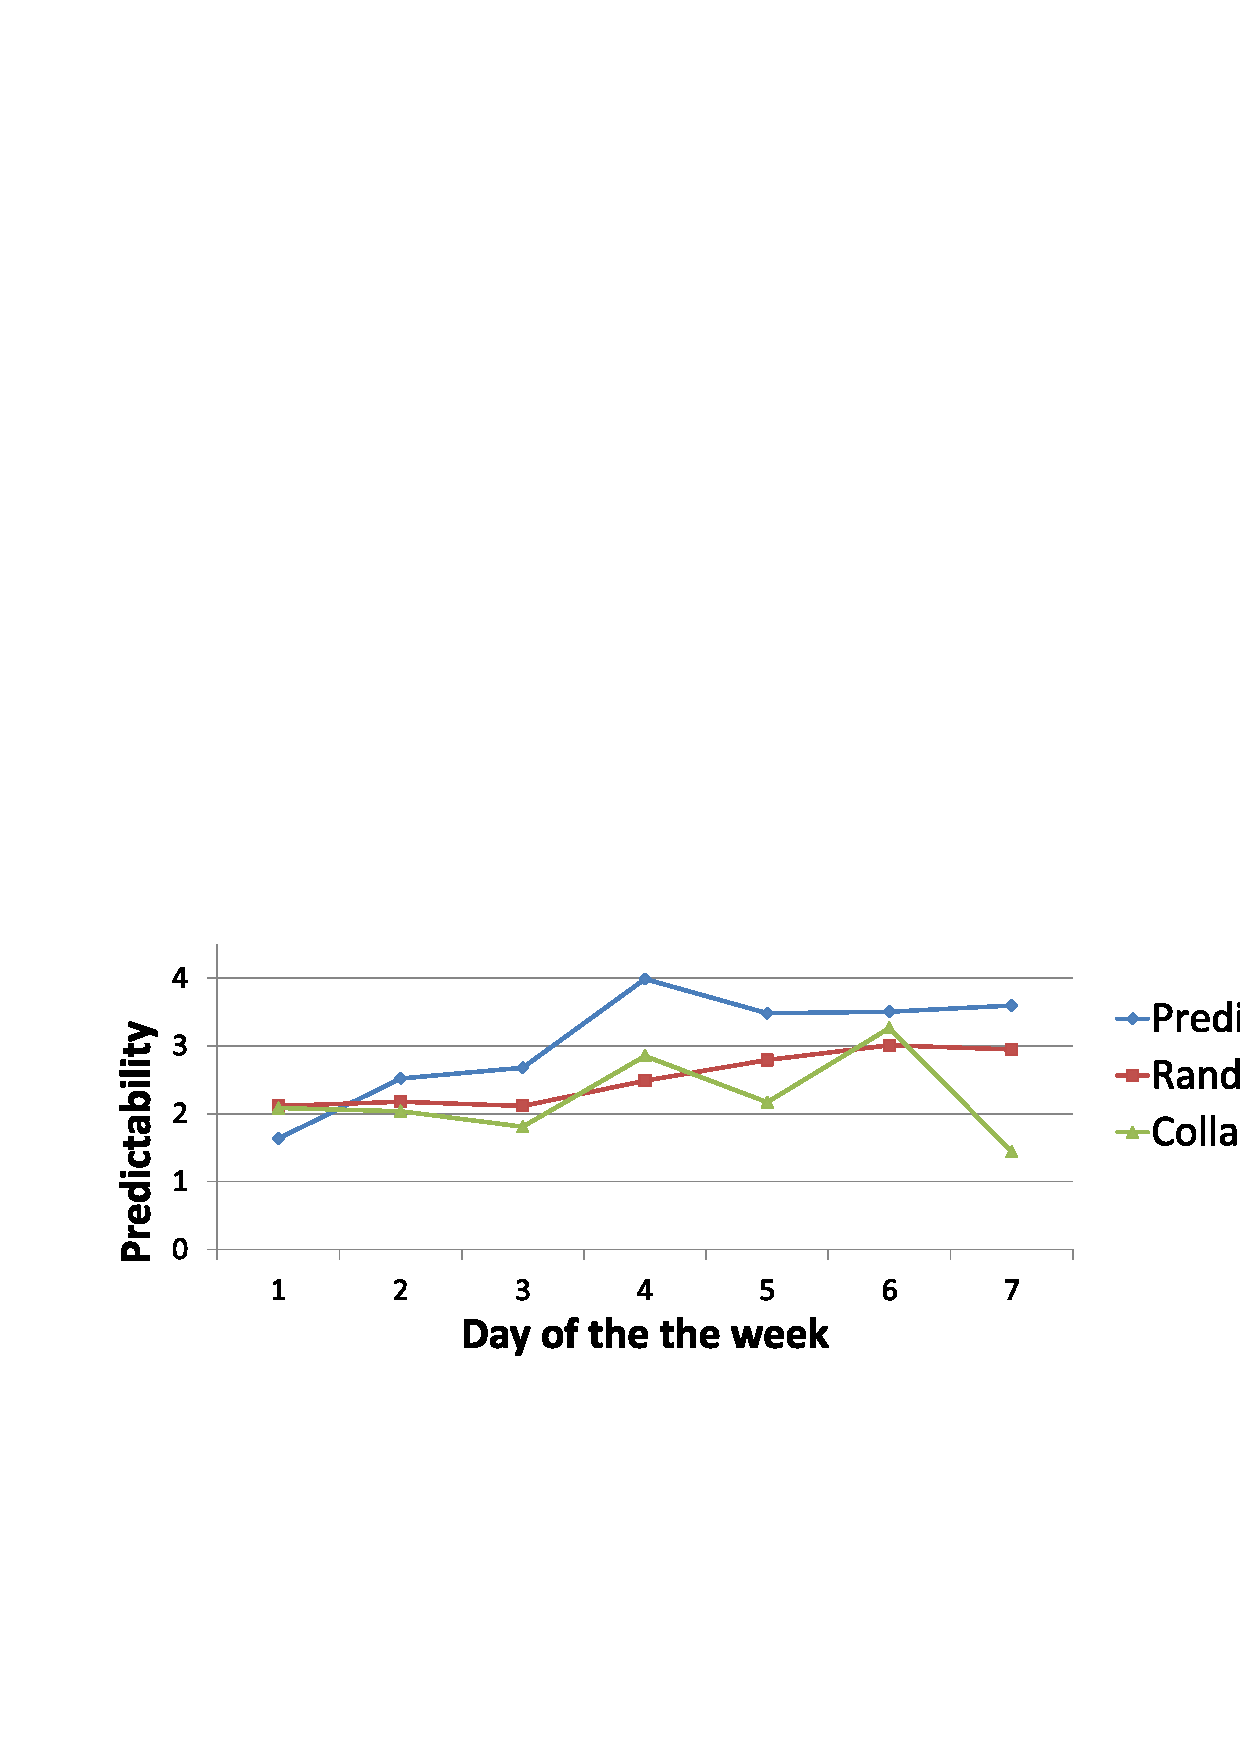
\includegraphics[width=0.48\columnwidth]{figures/precision.pdf}}
	\subfigure[]{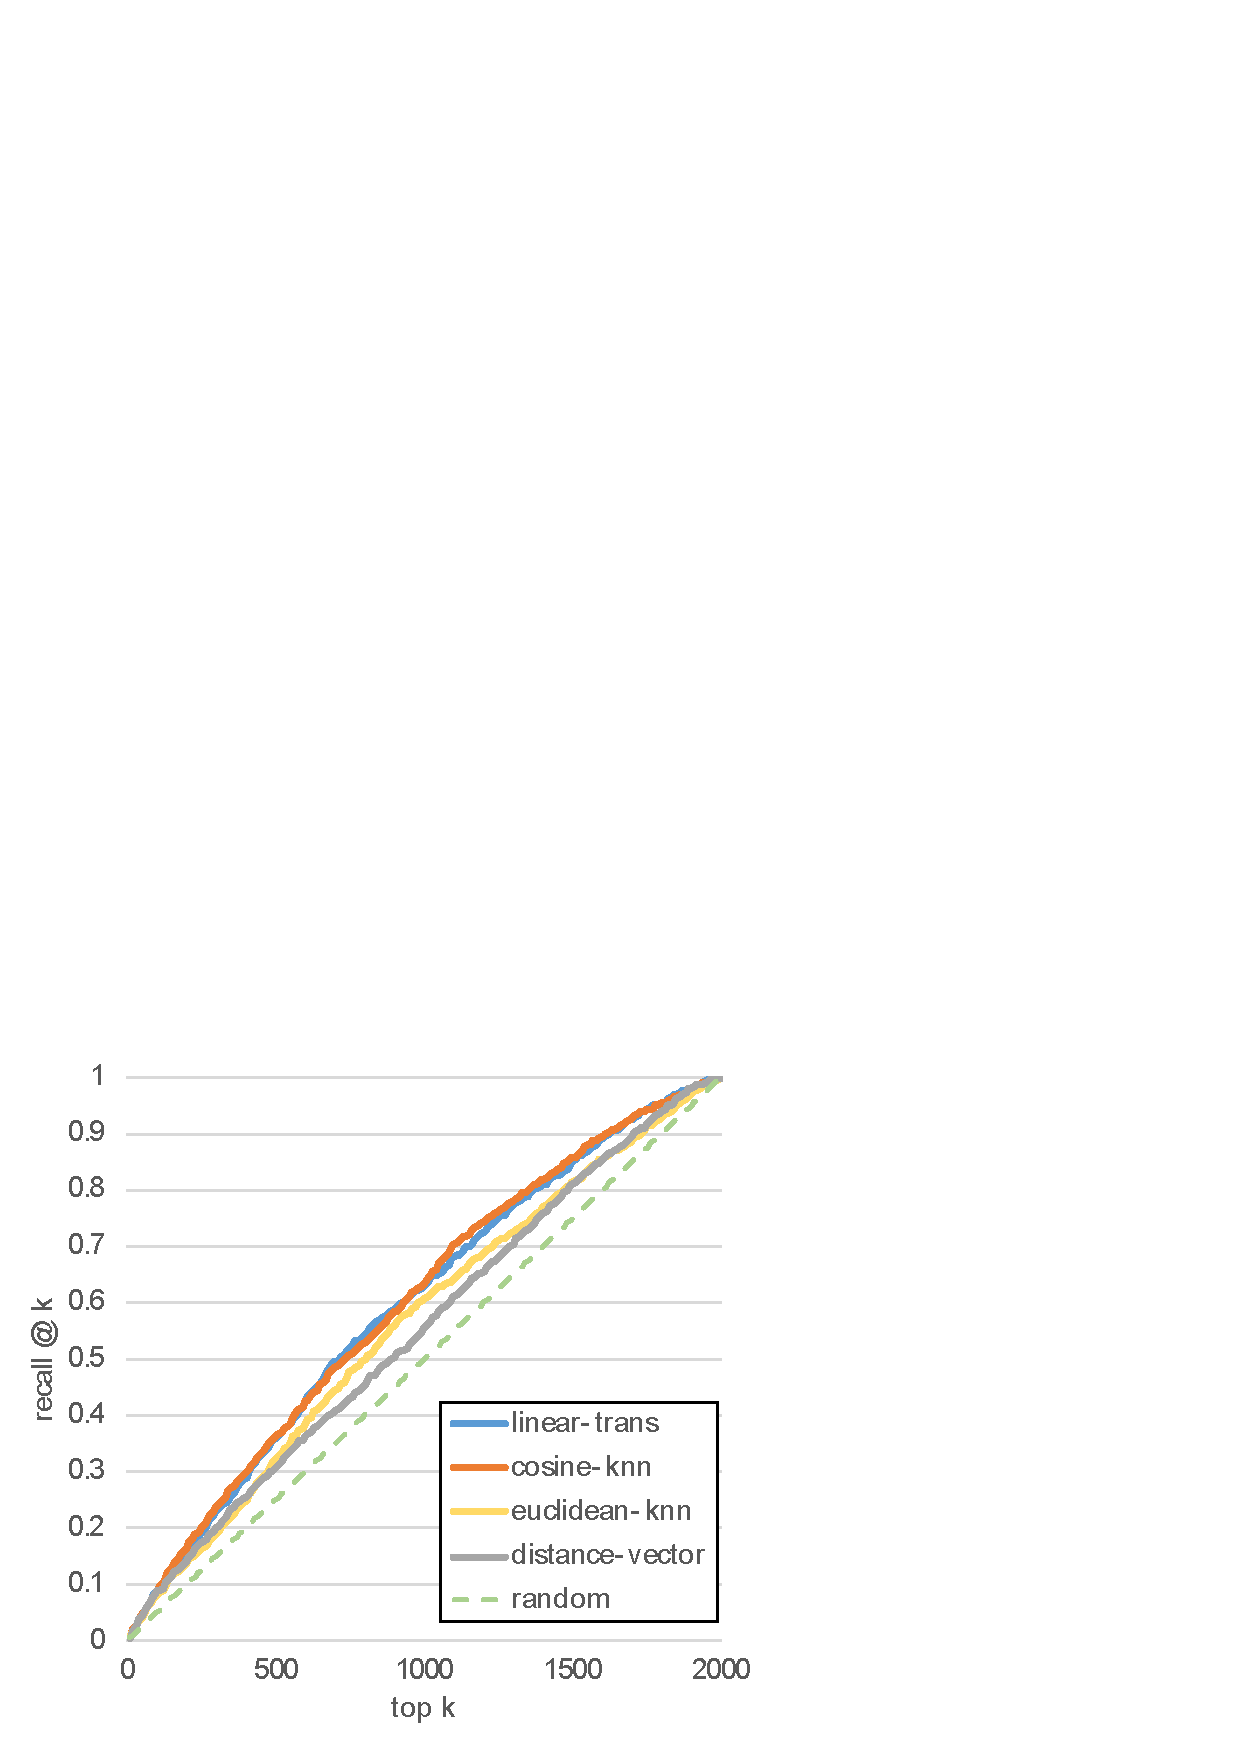
\includegraphics[width=0.48\columnwidth]{figures/recall.pdf}}
	\subfigure[]{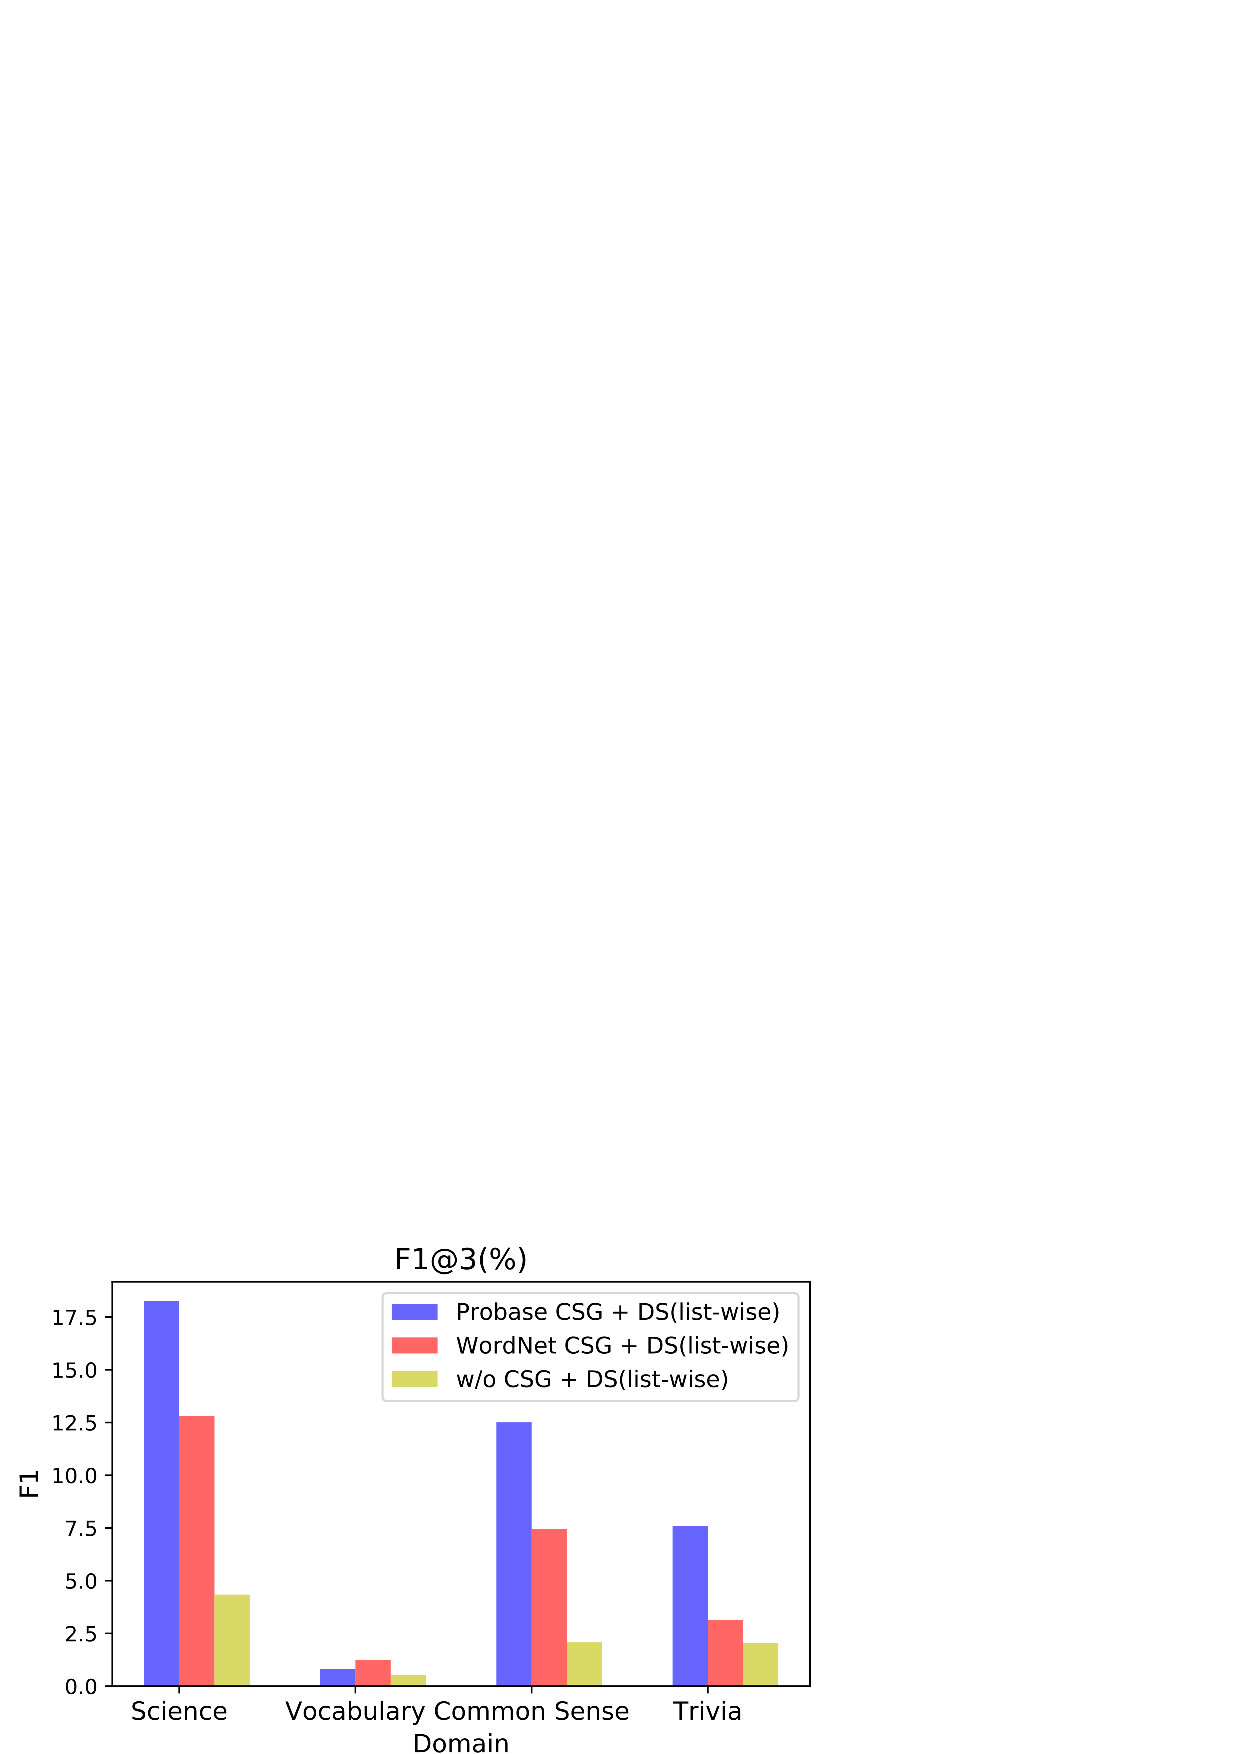
\includegraphics[width=0.48\columnwidth]{figures/f1.pdf}}
	\subfigure[]{\includegraphics[width=0.48\columnwidth]{figures/multi_grained.pdf}}
	\caption{(a)(b)(c) Learning trends of different methods.
			(d) Result of different cascade connection types in DCMTL.}
	\label{fig:learning_curve}
	\vspace{-10pt}
\end{figure}
%\begin{figure}[h]
%	\centering
%	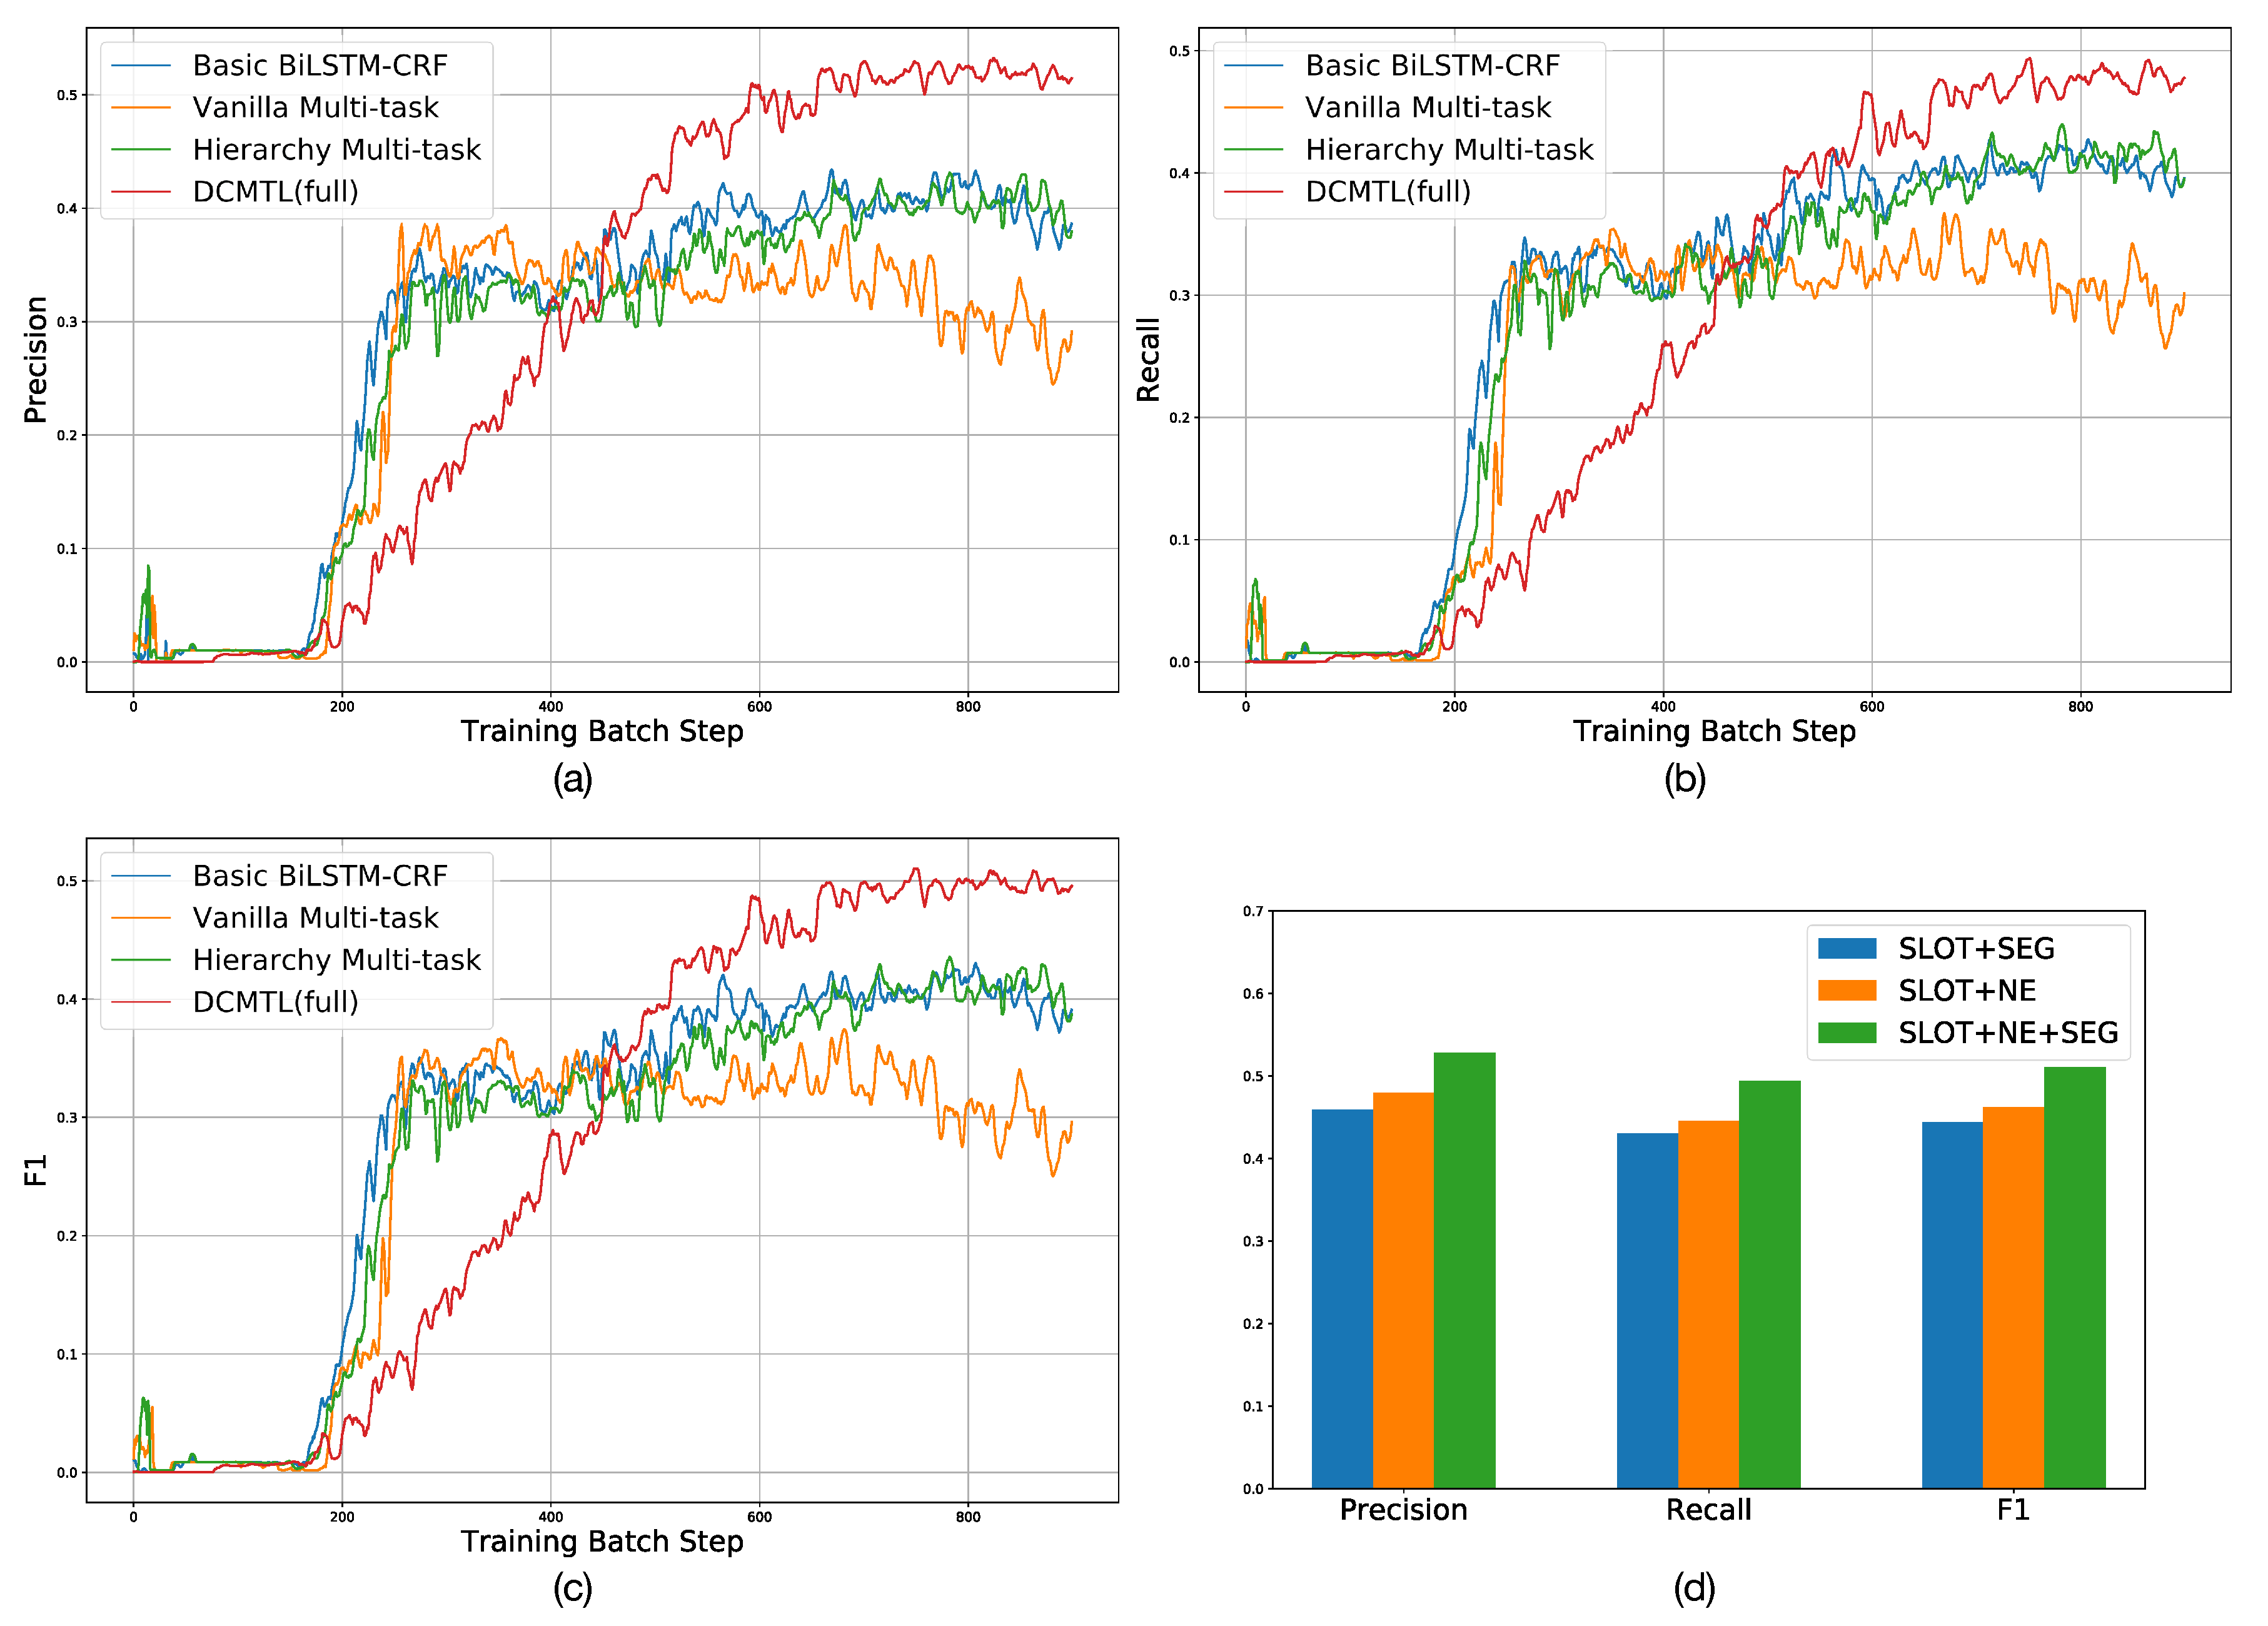
\epsfig{file=figures/learning_curve.eps, width=1.0\columnwidth}
%	\caption{(a)(b)(c) Learning trends of different methods.
%		(d) Result of different cascade connection types in DCMTL.}
%	\label{fig:learning_curve}
%	\vspace{-10pt}
%\end{figure}

%{\color{red}[[Modification Start]]}
To make our experiments more solid, 
we implement two models with the best performance on ATIS dataset: 
Sequential CNN \cite{vu2016sequential} (Sequence Labeling based) and Neural Sequence Chunking \cite{zhai2017neural} (Encoder-Decoder based).
They get XXX and XXX F1 scores respectively, and our DCMTL model outperforms both (see \tabref{tab:eval_ECSGA}).
%{\color{red}[[Modification End]]}
%\begin{table}[th]
%	\centering
%	\scriptsize
%	\begin{tabular}{c|c|c|c}
%		\toprule
%		Methods & Sequential CNN & Neural Sequence Chunking & DCMTL \\
%		\midrule
%		F1 &  &  & \textbf{0.5105} \\
%		\bottomrule
%	\end{tabular}
%	\caption{Comparison with published results on the ECSGA dataset.}
%	\label{tab:eval_ECSGA_SOTA}
%	\vspace{-10pt}
%\end{table}

\noindent
\textbf{Ablation Test:}
We also investigate how our model DCMTL performs 
with or without cascade and residual connections.
As shown in \tabref{tab:eval_ECSGA},
F1 score increases from 0.4840 to 0.5105 when residual connection is applied,
which verifies its benefit.
If we remove cascade connection from DCMTL,
the model actually degenerates into hierarchy multi-task model with residual connection.
From the table we find that it performs better than basic hierarchy multi-task model.
Meanwhile, we can conclude that 
cascade connection plays a more important role than residual connection in our DCMTL model.

Furthermore, 
we explore how DCMTL performs with different cascade connection methods.
We compare three different types of cascade connection 
illustrated in \figref{fig:cascade_connection_type}(a):
\begin{enumerate}[1.]
\item Segment labeling skipped to slot filling (SLOT+SEG).
\item Named entity labeling directly connected to slot filling (SLOT+NE).
\item Segment labeling, named entity labeling and slot filling in sequence (SLOT+NE+SEG).
\end{enumerate}
From \figref{fig:learning_curve}(d),
we find that cascade connection with type 3 
performs the best
and then with type 2,
while cascade method with skipped connection (type 1) performs the worst.
Therefore, we design the networks 
with a cascade connection in a hierarchical fashion
and do not apply skipped connection for the cascade 
inputs (\figref{fig:cascade_connection_type}(b)).
%\KZ{Can you speculate why type 3 and 2 are better than 1?}
This phenomenon here may also be proved by our case study above.
Slot filling performance with pre-known named entity type is 
much better than with pre-known segment type
(rows with * in \tabref{tab:eval_ECSGA}).
\begin{figure}[h]
	\centering
	\subfigure[]{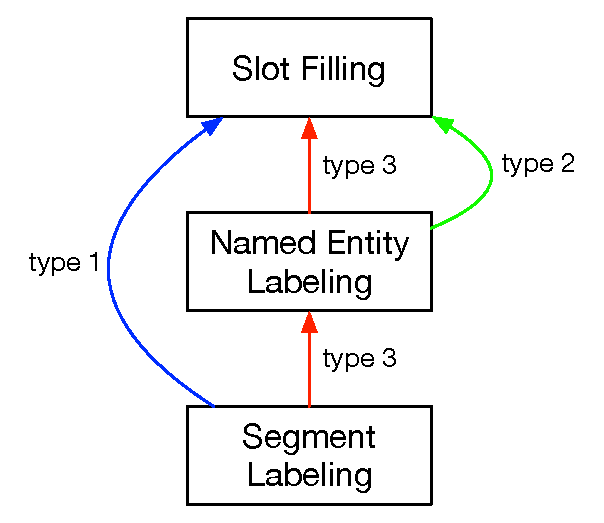
\includegraphics[width=0.48\columnwidth]{figures/cascade_connection_show.eps}}
	\subfigure[]{\includegraphics[width=0.48\columnwidth]{figures/cascade_connection_type.eps}}
	\caption{(a) Three types of cascade connection in our experiment.
			(b) Comparison between hierarchical and skipped cascade connection.}
	\label{fig:cascade_connection_type}
	\vspace{-10pt}
\end{figure}
%\begin{figure}[t]
%	\centering
%	\epsfig{file=figures/cascade_connection_type.eps, width=1.0\columnwidth}
%	\caption{(a) Three types of cascade connection in our experiment.
%	(b) Comparison between hierarchical and skipped cascade connection.}
%	\label{fig:cascade_connection_type}
%	\vspace{-10pt}
%\end{figure}

\subsection{Case Study}
We deploy DCMTL and baseline model (BiLSTM-CRF) on the online E-commerce Shopping Guide Assistant
and then analyze user query log.
Take slot labeling result of term ``一字领 (boat neckline)'' as an example 
(\tabref{tab:case_study}).
DCMTL label the whole trunk as a \textbf{Neckline Style},
while the baseline model splits it into two trunks (``一字'' and ``领'') and label ``一字'' as a \textbf{Contour Style}.
The reason may be that without knowing the segment information,
the prediction of slot labels 
could be disturbed by some similar terms such as ``A字 (A-line)'' which is another \textbf{Contour Style}.

We also extract terms from online user query log which are labeled as \textbf{Neckline\_Style} by DCMTL and show them in \tabref{tab:show_case}.
We find that our model can recognize 
the semantic attributes of user queries reasonably,
which is essential for \emph{Query Rewrite} and \emph{Dialog State Tracking} in E-commerce Shopping Guide Assistant system.

\begin{table}[h]
	\centering
	\scriptsize
	\begin{tabular}{c|c|c|c|c}
		\toprule
		\multicolumn{2}{c|}{\multirow{2}{*}{Term}} & 一 & 字 & 领  \\
		\cmidrule{3-5}
		\multicolumn{2}{c|}{} & \multicolumn{3}{c}{\emph{boat neckline}} \\
		\midrule
		\multirow{2}{*}{DCMTL} & Segment Label & \textbf{B} & \textbf{I} & \textbf{I} \\
		\cmidrule{2-5}
		& Slot Label & \textbf{B-NS} & \textbf{I-NS} & \textbf{I-NS} \\
		\midrule
	 	\multirow{2}{*}{Baseline} & Segment Label & \textbf{B} & \textbf{I} & \textbf{B} \\
		\cmidrule{2-5}
		& Slot Label & \textbf{B-CS} & \textbf{I-CS} & \textbf{B-NS} \\
		\bottomrule
	\end{tabular}
	\caption{Case study for term ``一字领 (boat neckline)'' in online query.
		In slot labels, \textbf{NS} is short for \textbf{Neckline\_Style}
		and \textbf{CS} is short for \textbf{Contour\_Style}.}
	\label{tab:case_study}
	\vspace{-10pt}
\end{table}

\begin{table}[h]
	\centering
	\scriptsize
	\begin{tabular}{|l|}
		\hline
			保罗领 (Polo neckline) / 一字领 (boat neckline) / 翻领 (lapel)\\
			衬衫领 (shirt collar) / V字领 (V-neck) / 深V领 (deep V-neck) \\
			圆领 (round collar) / 立领 (stand collar) / 鸡心领 (sweetheart neckline) \\
			荷叶边领 (lotus leaf collar) / 方口领 (square collar) / 花瓣领 (petal collar) \\
			水滴领 (drop collar) / 复古领 (vintage collar) / 半领 (half collar) \\
			飘带领 (floating collar) / 和服领 (kimono collar) / 中式领 (chinese collar) \\
			梯形领 (trapezoid collar) / 宽领 (wide collar) / 平领 (horizontal collar) \\
			水手领 (sailor collar) / 珍珠领 (pearl collar) / 花领 (flower collar) \\
			波浪领 (wave collar) / 尖领 (pointed collar) / 交叉领 (cross collar) \\
		\hline
	\end{tabular}
	\caption{Example terms slotted as \textbf{Neckline\_Style}.}
	\label{tab:show_case}
	\vspace{-10pt}
\end{table}
